\documentclass{beamer}

\usepackage{graphicx}
\usepackage{amsmath}
\usepackage[utf8]{inputenc}
\usetheme{default}
\usefonttheme{serif} 

\title{Introduction to Solid Mechanics and Biomaterials}
\author{Laura Miller and Gemini Advanced}
\date{\today}

\begin{document}

\frame{\titlepage}

\begin{frame}{Resources}
  \begin{itemize}
    \item \href{https://www.youtube.com/watch?v=-1TlNJL93sc}{Boyce Griffith presents IBFE and some solid mechanics at the 23-minute mark.}
    \item \href{https://solidmechanics.org/contents.php}{Applied Mechanics of Solids (A.F. Bower)}
    \begin{itemize}
    \item Sections we will cover are 2.1.1-2.1.14, 2.2, 2.3, 3.1, 3.2.1-3.2.12, 3.5.
    \item We may add additional sections, but this is a good starting place.
    \end{itemize}
    \item \href{https://drive.google.com/drive/folders/1vkhrX0YInMm5pfUj3LcRA9TV0DZdFp1a?usp=sharing}{Intro to Solid Mechanics from Matea Santiago}    
  \end{itemize}
\end{frame}

\begin{frame}{What is Solid Mechanics?}
    \begin{itemize}
        \item Solid mechanics is the study of how solid materials deform and respond to external forces.
        \item It is a fundamental branch of mechanics with applications in engineering, materials science, and biomechanics.
        \item In this lecture, we'll focus on concepts relevant to the hybrid immersed boundary finite element method.
    \end{itemize}
\end{frame}

\begin{frame}{Review: Stress and Strain}
  \begin{itemize}
    \item \textbf{Stress ($\sigma$):} Force per unit area.
      \begin{itemize}
        \item $\sigma = \frac{F}{A}$
        \item Units: Pascals (Pa) or N/m$^2$
      \end{itemize}
    \item \textbf{Strain ($\epsilon$):} Deformation per unit length.
      \begin{itemize}
        \item $\epsilon = \frac{\Delta L}{L_0}$
        \item Unitless
      \end{itemize}
    \item Importance: Understanding how biomaterials respond to forces in biological environments.
  \end{itemize}
\end{frame}

\begin{frame}{Introduction to Stress and Strain in 1D}
    \begin{itemize}
        \item In one-dimensional systems, stress and strain describe the behavior of a material under load.
        \item Consider a bar or rod fixed at one end and subjected to a tensile force at the other.
    \end{itemize}
\end{frame}

\begin{frame}{Supporting Image}
    \begin{figure}
        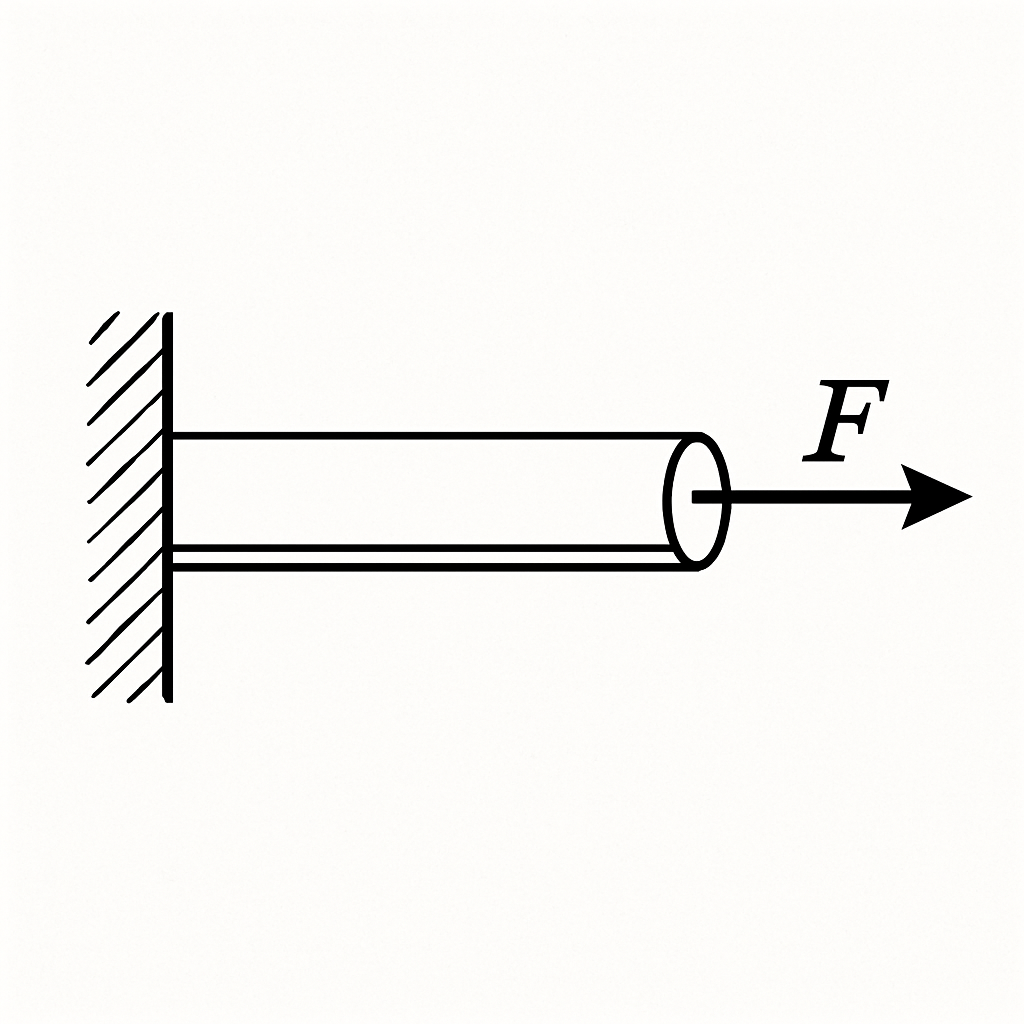
\includegraphics[width=0.5\textwidth]{../pictures/2-1/tensile-rod.png}
        \caption{An image of a rod fixed at one end and subjected to a tensile force at the other}
    \end{figure}
\end{frame}

\begin{frame}{Stress in 1D}
    \begin{itemize}
        \item Stress ($\sigma$) is defined as the force ($F$) applied per unit area ($A$) of the cross-section of the bar:
        \begin{equation*}
        \sigma = \frac{F}{A}
        \end{equation*}
    \end{itemize}
\end{frame}


\begin{frame}{Strain in 1D}
    \begin{itemize}
        \item Strain ($\epsilon$) is defined as the change in length ($\Delta L$) of the bar divided by its original length ($L_0$):
        \begin{equation*}
        \epsilon = \frac{\Delta L}{L_0}
        \end{equation*}
    \end{itemize}
\end{frame}

\begin{frame}{Stress-Strain Relationship in 1D}
    \begin{itemize}
        \item The relationship between stress and strain is described by the material's constitutive law.
        \item For a linear elastic material, Hooke's law applies:
        \begin{equation*}
        \sigma = E \epsilon
        \end{equation*}
        where $E$ is the Young's modulus of the material.
    \end{itemize}
\end{frame}

\begin{frame}{Stress and Strain}
    \begin{figure}
        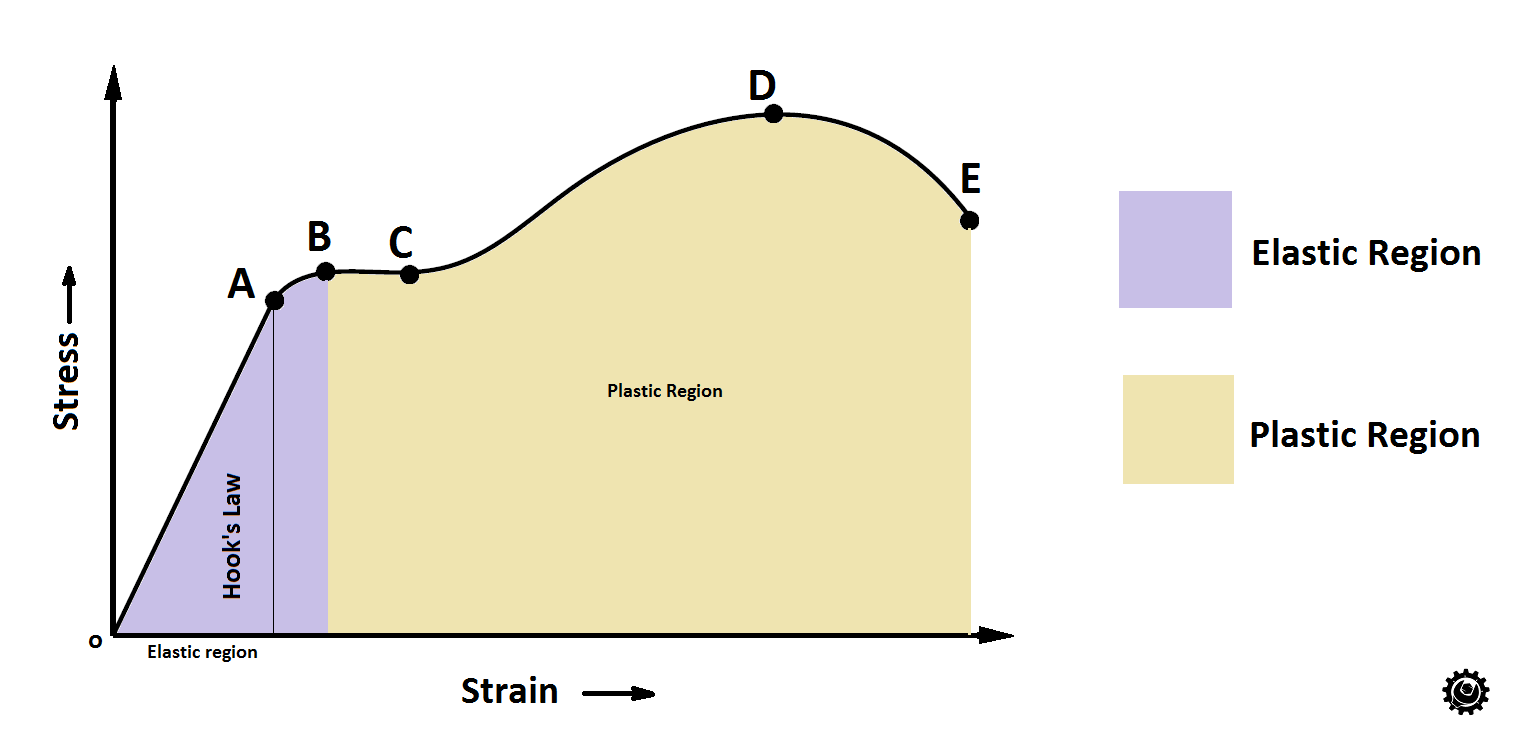
\includegraphics[width=0.9\textwidth]{../pictures/stress-strain-curve-001.png}
        \caption{Stress vs. Strain.
        Note that the linear part of the graph represents a Hookean material that follows Hook's law. The plastic region is the area on a stress-strain curve that represents the material's behavior after it has yielded.

}
    \end{figure}
\end{frame}

\begin{frame}{Multidimensional Stress and Strain}
    \begin{itemize}
        \item Real-world problems often involve multidimensional loading and deformation, beyond the 1D case.
        \item In higher dimensions, stress and strain become tensor quantities, with both magnitude and multiple directions.
        \item This complexity arises from forces acting on a body in various directions, causing deformation in multiple ways.
        \item Stress and strain tensors are needed to fully describe the state of stress and strain in multidimensional settings.
        \item These tensors capture the complex interplay of forces and deformations, providing a complete picture of material behavior.
    \end{itemize}
\end{frame}

\begin{frame}{Types of Stress}
  \begin{itemize}
    \item \textbf{Tensile Stress:} Stretching (e.g., ligament under tension).
    \item \textbf{Compressive Stress:} Squeezing (e.g., bone under load).
    \item \textbf{Shear Stress:} Tangential force (e.g., sliding of tissue layers).
  \end{itemize}
\end{frame}

\begin{frame}{Loading Definitions}
Loading refers to the application of external forces or moments to a solid body. These applied forces and moments cause internal stresses and strains within the material, which can lead to deformation or even failure.
  \begin{itemize}
    \item \textbf{Axial Loading:} Force along the longitudinal axis (tensile or compressive).
    \item \textbf{Bending:} Application of a moment, inducing tensile and compressive stresses. Moment: $M=Fd$
    \item \textbf{Torsion:} Twisting, inducing shear stress. Torque: $T=Fr$
  \end{itemize}
\end{frame}

\begin{frame}{Supporting Image}
    \begin{figure}
        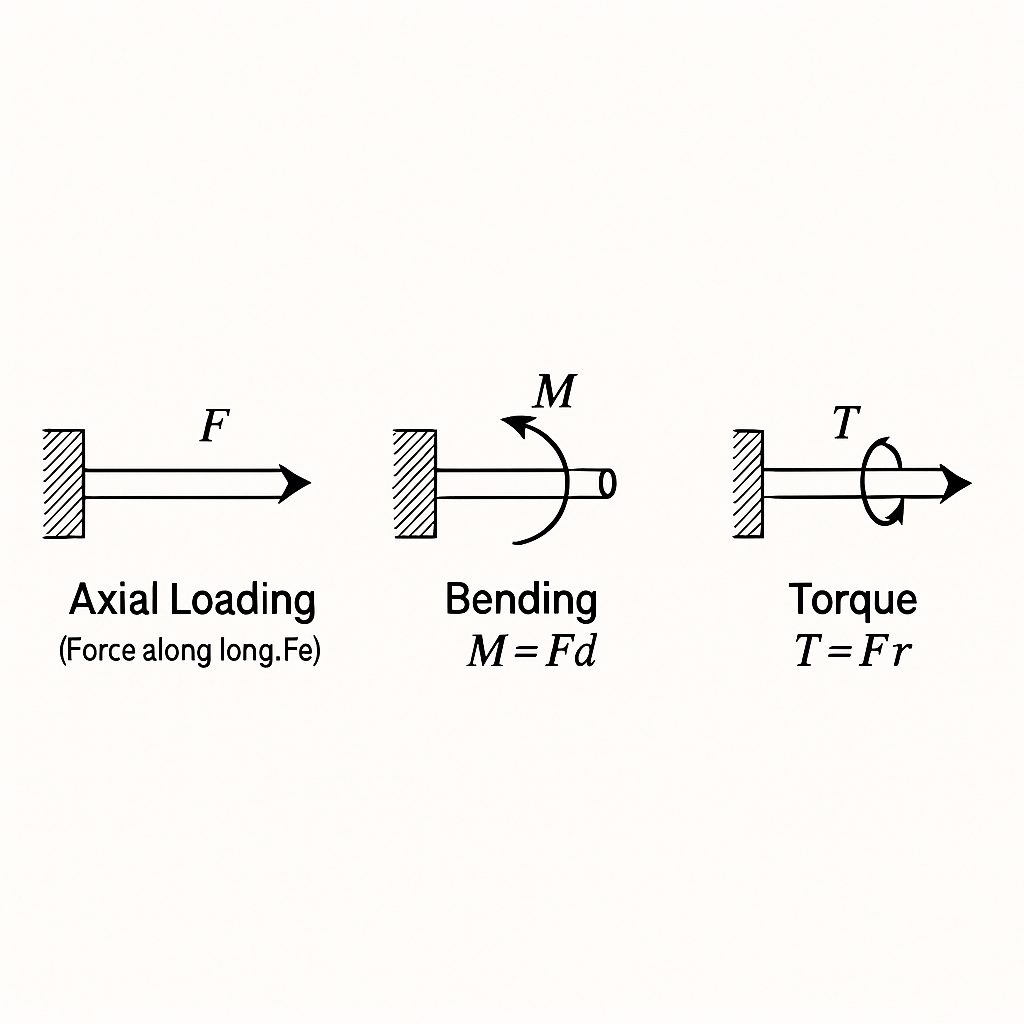
\includegraphics[width=0.65\textwidth]{../pictures/2-1/Moment-Torque.png}
        \caption{An image of a rod fixed at one end and subjected to an axial loading, bending with moment $M$, and torque $T$.}
    \end{figure}
\end{frame}

\begin{frame}{Material Properties: Young's Modulus}
  \begin{itemize}
    \item \textbf{Young's Modulus (E):} Stiffness of a material.
      \begin{itemize}
        \item $\sigma = E\epsilon$ (Linear elastic region)
        \item High E: Stiff material (e.g., cortical bone).
        \item Low E: Flexible material (e.g., soft tissue).
      \end{itemize}
  \end{itemize}
\end{frame}

\begin{frame}{Material Properties: Poisson's Ratio}
  \begin{itemize}
    \item \textbf{Poisson's Ratio ($\nu$):} Ratio of lateral to axial strain.
      \begin{itemize}
        \item $\nu = -\frac{\epsilon_{lateral}}{\epsilon_{axial}}$
        \item Affects volume changes under load.
      \end{itemize}
  \end{itemize}
      \begin{figure}
        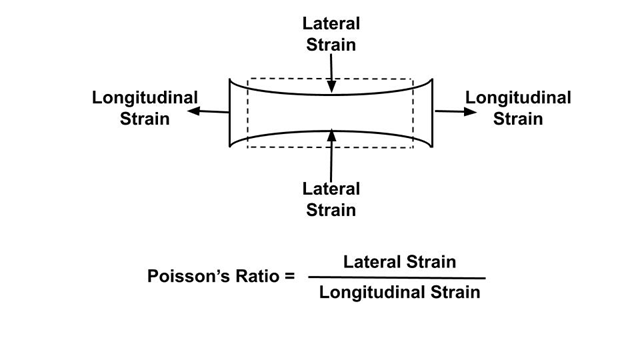
\includegraphics[width=0.65\textwidth]{../pictures/2-1/poisson.png}
    \end{figure}
\end{frame}

\begin{frame}{Material Properties: Yield Strength}
  \begin{itemize}
    \item \textbf{Yield Strength ($\sigma_y$):} Stress at which permanent deformation occurs (important for implant design).
  \end{itemize}
        \begin{figure}
        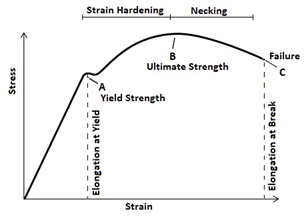
\includegraphics[width=0.5\textwidth]{../pictures/2-1/yield-strength.png}
    \end{figure}
\end{frame}

\begin{frame}{Material Behavior}
  \begin{itemize}
    \item \textbf{Linear Elastic:} Stress proportional to strain. (Example - steel, aluminum)
    \item \textbf{Non-linear:} Stress-strain relationship is not linear. (Example - Rubber)
    \item \textbf{Viscoelastic:} Time-dependent deformation (creep and relaxation, common in biological tissues)
  \end{itemize}
\end{frame}

\begin{frame}{Pressure and Traction}
  \begin{itemize}
    \item \textbf{Pressure:} Normal force applied over a surface area, acting perpendicular to the surface. $P = \frac{F_n}{A}$ (Pascals). Example: Fluid pressure on tissue.
    \item \textbf{Traction:} Force per unit area acting on a surface, with normal and tangential components (frictional forces). Example: Shear forces between tissue layers.
    \item \textbf{Key Difference:} Pressure is always normal, while traction can have both normal and tangential components.
  \end{itemize}
\end{frame}

\begin{frame}{Boundary Conditions and Loading}
  \begin{itemize}
    \item \textbf{Types of Mechanical Loads:}
      \begin{enumerate}
        \item Prescribed displacements or motion.
        \item Pressure or traction on boundaries.
        \item Mixed displacement and traction.
        \item Body forces (gravity, electromagnetic).
        \item Contact between solids (or self-contact).
        \item Thermal or material process-induced stresses.
      \end{enumerate}
  \end{itemize}
\end{frame}

\begin{frame}{Boundary Condition Rules}
  \begin{itemize}
    \item \textbf{3D:} 3 components of displacement or traction (not both) at each boundary point.
    \item \textbf{2D:} 2 components of displacement or traction at each boundary point.
    \item Static problems with traction only: Total external force must be zero.
  \end{itemize}
\end{frame}

\begin{frame}{Boundary Conditions: Practical Considerations}
  \begin{itemize}
    \item Loading can be complex (earthquakes, wind, contact).
    \item Requires accurate estimation of loading parameters (acceleration, pressure, friction).
    \item Nano-scale or biological applications: Consider attractive forces.
  \end{itemize}
\end{frame}

\begin{frame}{Material Models}
    \begin{itemize}
        \item \textbf{Isotropic Linear Elasticity:} Material properties are the same in all directions. $\sigma = C \epsilon$ (stiffness tensor), simplified to $\sigma = E \epsilon$ (1D).
        \item \textbf{Anisotropic Linear Elasticity:} Material properties vary with direction (e.g., bone). Requires a full stiffness tensor.
        \item \textbf{Hyperelasticity:} Large deformations, non-linear elastic behavior. Strain energy function $W(\epsilon)$ describes the material response (e.g., soft tissues).
        \item \textbf{Viscoelasticity:} Time-dependent deformation. Stress depends on strain rate. Generalized Maxwell or Kelvin-Voigt models. $\sigma(t) = \int_{-\infty}^{t} G(t-\tau) \frac{d\epsilon(\tau)}{d\tau} d\tau$
        \item \textbf{Viscoplasticity:} Time-dependent plastic (permanent) deformation. Yield stress depends on strain rate (e.g., bone remodeling).
    \end{itemize}
\end{frame}

\begin{frame}{Applications in Biomaterials}
  \begin{itemize}
    \item Implant design: Matching mechanical properties to host tissue.
    \item Tissue engineering: Understanding cell-matrix interactions.
    \item Biomechanical compatibility: Minimizing stress shielding.
    \item Long-term stability: Predicting implant lifespan.
  \end{itemize}
\end{frame}


\end{document}